\documentclass[tikz, a4paper,12pt]{extreport}
\usepackage{preamble}


\usetikzlibrary{calc}
\usetikzlibrary{intersections}
\usetikzlibrary{angles}
\usetikzlibrary{quotes}

\begin{document}
  \begin{center}
    \textbf{Дальневосточный федеральный университет}\par
    Центр проектной деятельности\par
    \textbf{Федоров Константин Сергеевич}\par
    \textit{17.04.2018}
  \end{center}
  \chapter{Описание проекта}\par
  \section{Общая постановка задачи}\par
  \noindent\indent  Разработать мат. модель и провести численное моделирование
  действия солнечного давления на солнечный парус космического аппарата
  класса "Cubesat".
  \section{Частная постановка задачи}\par
    \noindent\indent Необходимо реализовать два плагина, совместимых с программой <<Sputnix Modeller>>:
    \begin{itemize}
      \item по расчету сил и моментов от солнечного давления,
      \item реализующий закон управления парусом (по сути, задающий требуемй
      угол падения солнечных лучей на полотно в зависимости от текущих
      параметров ориентации)
    \end{itemize}
    \subsection{Плагин 1}\par
    \noindent\indent Исходные данные для модели/плагина 1:
    \begin{itemize}
      \item параметры орбиты,
      \item положение солнца относительно спутника (в виде единичного орта в
      связанной с аппаратом системе координат),
      \item положение паруса относительно солнца (парус может поворачиваться
      относительно спутника)
      \item на свету или в тени находится аппарат
      \item конструкция аппарата (моменты инерции, координаты центра давления
      относительно центра масс),
      \item конструкция паруса (для начала - сплошное полотно с различными
      коэффициентами отражения и поглощения; другие вариант - лопасти
      заданной геометрии)
    \end{itemize}\par
    Выходные данные:
    \begin{itemize}
      \item момент
      \item сила
    \end{itemize}
    \subsection{Плагин 2}\par
    \noindent\indent Входные данные:
    \begin{itemize}
      \item текущие параметры ориентации спутника относительно Солнца (углы,
      угловые скорости)
    \end{itemize}\par
    Выходные данные:
    \begin{itemize}
      \item требуемое программное изменение угла поворота паруса/спутника
    \end{itemize}
  \chapter{Преобразование входных данных}\par
  \noindent\indent Будем предполагать, что солнечный парус имеет простую (не композитную) плоскую конструкцию.
  Для перехода от простой к композитной конструкции будем рассчитывать итоговые величины
  как интегральную сумму по всем "компонентам" паруса (будем считать их, как дополнительные солнечные паруса).
  \section{Положение спутника относительно Земли}
  \noindent\indent Первоначально, мы имеем орбитальные параметры спутника:
  \begin{itemize}
    \item большая полуось орбиты, $a$,
    \item эксцентриситет орбиты, $e$,
    \item наклонение орбиты, $i$,
    \item долгота восходящего узла орбиты, $\Omega$,
    \item аргумент перицентра орбиты, $\omega$,
    \item истинная аномалия, $\nu$
  \end{itemize}
  \setlength\intextsep{0pt}
  \begin{figure}[h]
    \centering
    \begin{minipage}[t]{0.35\textwidth}
      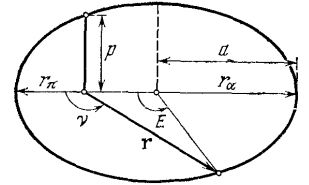
\includegraphics[width=\linewidth]{Orbit_2D.png}
      \caption{Кеплеровская эллиптическая орбита}
      \label{fig:KeplerOrbit2D}
    \end{minipage}
    \hspace{2 cm}
    \begin{minipage}[t]{0.35\textwidth}
      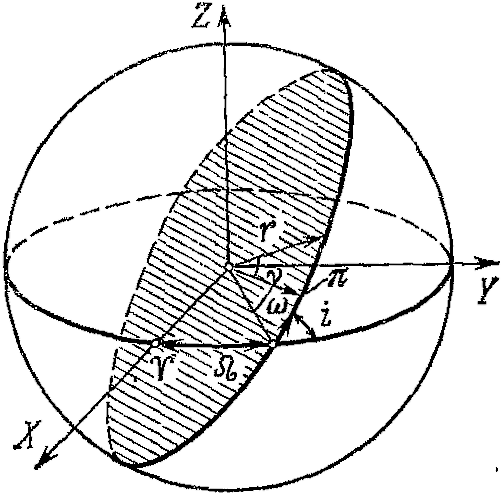
\includegraphics[width=\linewidth]{Orbit_Kepler.png}
      \caption{Кеплеровы элементы}
      \label{fig:KeplerOrbitParameters}
    \end{minipage}
  \end{figure}
  \setlength\intextsep{0pt}
  \subsection{Положение спутника на орбите Земли}
  \noindent\indent Исходя из данных параметров, для рассчета положения спутника в каждый момент времени
  (при условии учитывания лишь гравитационных сил, возникающих между Землей и спутником)
  мы можем воспользоваться законом площадей:
  \begin{equation}
    r^2 \frac{d\nu}{dt} = \sqrt{\mu p},
  \end{equation}\par
  Также введем такую величину, как <<эксцентрическая аномалия>> $E$, что связана с $\nu$ соотношением:
  \begin{equation}
    \cos{\nu} = \frac{\cos{E} - e}{1 - e\cos{E}}, \\
    \sin{\nu} = \frac{\sin{E}}{1 - e\cos{E}}\sqrt{1 - e^2},
  \end{equation}
  причем
  \begin{equation}
    r = a(1 - e\sin{E})
  \end{equation}\par
  Эксцентрическая аномалия $E$ связана со временем t уравнением Кеплера:
  \begin{equation} \label{eq:Et}
    E - e\sin{E} = n(t - t^*),
  \end{equation}
  где $n = \sqrt{\mu/a^3}$ - так называемое среднее движение; постоянная t*
  обозначает момент прохождения через перигей орбиты. Также из \ref{eq:Et} следует,
  что период обращения спутника по орбите
  \begin{equation}
    T = 2\pi\sqrt{a^3/\mu}.
  \end{equation}\par
  Уравение \ref{eq:Et} не решается аналитически, поэтому для её вычисления будем использовать
  один из алгоритмов численного решения уравений, к примеру, метод Эйлера:
  \begin{equation}
    \begin{aligned}
      & E_{k+1} = e\sin{E_k} + M, \\
      & M = n(t - t^*)
    \end{aligned}
  \end{equation}
  Тем самым, положение спутника в каждый момент времени в орбитальной системе координат
  будет вычисляться по формуле:
  \begin{equation}
    \begin{aligned}
      & \vec{r}_{earth\_sat/orbit} = r \cdot [\cos{\nu}, \sin{\nu}, 0], \\
      & r = a(1 - e\sin{E})
    \end{aligned}
  \end{equation}
  Переводим это в глобальную систему координат, предполгая, что мы имеем \textit{базис орбиты}\footnote{
    Его возможно определить при известном начальном положении спутника (в момент вывода на орбиту)
  }, и получаем положение спутника в глобальной системе координат
  \begin{equation} \label{eq:REarthSat}
    \hat{\vec{r}}_{earth\_sat} = R_{orbit\_global} \cdot \vec{r}_{earth\_sat/orbit}
  \end{equation}
  \subsection{Учет неоднородности Земли}
  \noindent\indent Учет показателей долготы восходящего узла орбиты ($\Omega$) и аргумент перицентра
  орбиты ($\omega$) дает возможность получить более точную картину изменения положения спутника.
  Если быть более точным, то они определяют как будет изменятся траектория орбиты в пространстве.
  Ссылаясь на книгу Белецкого В. В. <<Очерки о движении космических тел>>, наибольший эффект
  на изменение орбиты оказывает сплюснутость Земли к полюсам. В указанной уже книге, для
  рассчета данного эффекта, используется разложение силовой функции Земли через полиномы Лежандра:
  \begin{equation}
    \begin{aligned}
      & U = \frac{\mu}{r} \cdot \left\{1 + \sum\limits_{k=2}^{\infty}I_k\left(\frac{R}{r}\right)^k P_k(\sin{\phi})\right\}, \\
      & \mu = f M,
    \end{aligned}
  \end{equation}
  где $M$ - масса Земли,
  $f$ - универсальная постоянная тяготения,
  $R$ - экваториальный радиус Земли,
  $\phi$ - географическая широта точки.
  Коэффициенты $I_k$ имеют фиксированные безразмерные значения.
  Функция $P_k$ представляет собой полиномы Лежандра.\par
  Наибольший эффект оказывает член с коэффициентом $I_2 = -1082.2 \cdot 10^{-6}$. \par
  Опустив выкладку из упомянутой выше книги, сразу запишем итоговую систему ДУ:
  \begin{equation}
      \begin{cases}
        \frac{d\Omega}{d\tau} = \frac{3}{2}I_2\left(\frac{R}{p}\right)^2 \cos{i}, \\
        \frac{d\omega}{d\tau} = \frac{3}{4}I_2\left(\frac{R}{p}\right)^2(1 - 5\cos^2{i}),
      \end{cases}
  \end{equation}
  где $\tau = n \cdot t$ - безразмерное время.\par
  Решив данные ДУ, получим систему линейных уравнений:
  \begin{equation}
      \begin{cases}
        \hat{\Omega} = \frac{3}{2}I_2\left(\frac{R}{p}\right)^2 \cos{i} \cdot \tau + \Omega, \\
        \hat{\omega} = \frac{3}{4}I_2\left(\frac{R}{p}\right)^2(1 - 5\cos^2{i}) \cdot \tau + \omega,
      \end{cases}
  \end{equation}
  Применив данные уравнения к формуле \ref{eq:REarthSat}, первоначально получив
  из них матрицы(или кватернионы) поворота, получим более точное уравнение движения спутника в поле тяготения Земли:
  \begin{equation}
    \vec{r}_{earth\_sat} = R_{\hat{\Omega}} \cdot R_{\hat{\omega}} \cdot \hat{\vec{r}}_{earth\_sat}
  \end{equation}
  \section{Положение Солнца относительно солнечного паруса}
  \noindent\indent Первоначально, нам передается нормированный вектор, направленный от Солнца к спутнику $\vec{e}_{solar\_sat}$.
  Однако, нам необходим нормированный вектор, направленный от Солнца к центру масс солнечного
  паруса $\vec{e}_{solar\_sail}$.\par
  Предположим, что мы имеем координаты центра масс паруса относительно центра масс спутника ($x_{sail/sat} = T_{sat} \cdot x_{sail} = x_{sail} - x_{sat} = \vec{r}_{sat\_sail}$).
  Тогда необходимый вектор будет выведен по формуле:
  \begin{equation} \label{eq:ESolarSail}
    \vec{e}_{solar\_sail} = \frac{\vec{e}_{solar\_sat} + x_{sail/sat}}{||\vec{e}_{solar\_sat} + x_{sail/sat}||}
  \end{equation}
  % \setlength\intextsep{0pt}
  \begin{figure}[!h]%{r}{0pt}
    \centering
    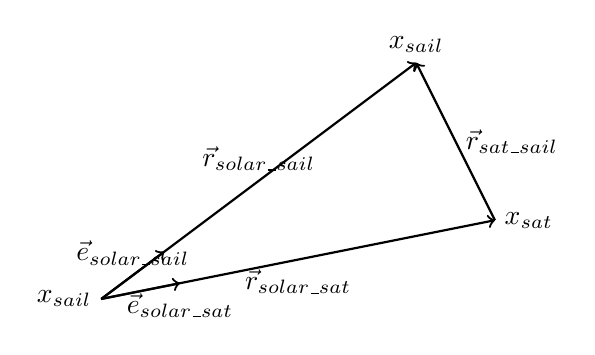
\begin{tikzpicture}
      \draw[.] (0,0) node[left] {$x_{sail}$};
      \draw[thick, ->] (0,0) -- node[below] {$\vec{r}_{solar\_sat}$} (5,1);
      \draw[thick, ->] (0,0) -- (1, 0.2) node[below] {$\vec{e}_{solar\_sat}$};
      \draw[.] (5,1) node[right] {$x_{sat}$};
      \draw[thick, ->] (5,1) -- node[right] {$\vec{r}_{sat\_sail}$} (4, 3);
      \draw[.] (4,3) node[above] {$x_{sail}$};
      \draw[thick, ->] (0,0) -- node[above] {$\vec{r}_{solar\_sail}$} (4, 3);
      \draw[thick, ->] (0,0) -- node[above] {$\vec{e}_{solar\_sail}$} (0.8, 0.6);
    \end{tikzpicture}
    \caption{Взаимное расположение объектов из \ref{eq:ESolarSail}}
    \label{fig:SolarSatSailSystem}
  \end{figure}
  % \setlength\intextsep{0pt}
  \section{<<Сила солнечного ветра>>}
  \noindent\indent
  % Предположим, что известны следующие величины:
  % \begin{itemize}
  %   \item общую массу аппарата ($m_{sat}$),
  %   \item площадь солнечного паруса ($\Omega_{sail}$),
  %   \item расстояние от центра Земли до спутника($r_{earth\_sat}$)
  %   \item вектор нормали паруса ($\vec{n}_{sail}$)
  %   \item нормированный вектор, направленный от Солнца к Земле ($\vec{e}_{solar\_earth}$)
  %   \item нормированный вектор, направленный от Земли к спутнику ($\vec{r}_{earth\_sat}$)
  % \end{itemize}\par
  Величина солнечного давления на расстоянии $r$ от Солнца высчитывается по следующей формуле:
  \begin{equation}
    P = \frac{S_0}{c}\left(\frac{r_0}{r}^2\right),
  \end{equation}
  где $S_0$ - солнечная постонная, равная $1368 \text{Вт}/\text{м}^2$, $c$ - скорость
  света в вакууме, равная приблизительно $3 \cdot 10^8 \text{м}/\text{с}$, $r_0$ -
  одна астрономическая единица ($~1.5 \cdot 10^{11} \text{м}$). Так на околоземной орбите
  давление света $P \approx 4.6 \cdot 10^{-6} \text{Н}/\text{м}^2$.\par
  Тогда, при условии полного зеркального отражения света поверхностью, сила $\vec{F}$,
  действующая на плоский парус с площадью отражения $\Omega$ и нормалью $\vec{n}$, будет равна:
  \begin{equation}
    \vec{F} = -2P\Omega\cos^2{(\alpha)}\vec{n},
  \end{equation}
  где $\alpha$ - угол между нормалью к поверхности паруса $\vec{n}$ и направляющим
  вектором падающего на парус солнечного излучения $\vec{e_r}$.

  \begin{figure}[!h]
    \centering
    \begin{tikzpicture}
      \coordinate (center) at (3, 0);
      \coordinate (norm) at (0, 0);
      \coordinate (eR) at (0.88, 2.12);
      \coordinate (revER) at (0.88, -2.12);

      \draw[line width=0.05mm, -] (3, -3) -- (3, 3);
      \draw[line width=0.05mm, ->] (center) -- node[above] {$\vec{n}$} (norm);
      \draw[line width=0.2mm, ->] (eR) -- node[above] {$\vec{e_r}$} (center);
      \draw[line width=0.2mm, ->] (center) -- (revER);

      \path (norm) -- (center) -- (eR)
      pic[%
        % "$\alpha$",%
        draw,%
        -,%
        red,%
        angle radius = 0.5cm,%
        angle eccentricity = 1.2]%
        {angle = eR--center--norm};
      \path (norm) -- (center) -- (revER)
      pic[%
        % "$\alpha$",%
        draw,%
        -,%
        red,%
        angle radius = 0.3cm,%
        angle eccentricity = 1.2]%
        {angle = norm--center--revER};
    \end{tikzpicture}
    \caption{Отражение света <<идеальным>> солнечным парусом}
    \label{fig:SimpleSailLightReflection}
  \end{figure}\par

  Однако, в реальности невозможно получить идеально отражающую поверхность, поэтому
  необходимо построить более общую модель паруса. В отличие от идеально отражающей
  поверхности, реальная может также отражать свет рассеиванием, поглощать свет и переизлучать
  свет в виде тепла с обеих сторон поверхности.\par
  Введем следующие оптические коэффициенты:
  \begin{itemize}
    \item $\mu$ -- коэффициент поглощения солнечного света парусом;
    \item $\nu$ -- коэффициент прозрачности паруса;
    \item $\rho$ -- общий коэффициент отражения солнечного света;
    \item $\rho_s$ -- коэффициент отражения солнечного света зеркально;
    \item $\rho_d$ -- коэффициент отражения солнечного света рассеиванием.
  \end{itemize}\par
  Отметим, что будут выполняться соотношения
  $
    \rho = \rho_s + \rho_d \\
    \mu + \rho + \nu = 1.
  $
  \begin{equation}
    s = \frac{\rho_s}{\rho}
  \end{equation}
  - отношение коэффициента отражения света зеркально к общему коэфиценту отражения;
  \begin{itemize}[label={}]
    \item $\epsilon_f$, $\epsilon_b$ -- коэффициенты переизлучения с передней и
    обратной стороны паруса соответственно;
    \item $B_f$, $B_b$ -- характеризуют угловое распределение излучения передней
    и обратной стороны паруса.
  \end{itemize}\par
  Тогда имеем:
  \begin{equation}
    \vec{F}_a = -P\Omega\mu\left(\frac{\epsilon_f B_f - \epsilon_b Bb}{\epsilon_f + \epsilon_b}(\vec{e}_r \cdot \vec{n})\vec{n} + |\vec{e}_r \cdot \vec{n}|\vec{e}_r\right)
  \end{equation}
  -- сила, возникающая при поглощении света;
  \begin{equation}
    \vec{F}_{rs} = -2P\Omega\rho_s(\vec{e}_r \cdot \vec{n})|\vec{e}_r \cdot \vec{n}|\vec{n}
  \end{equation}
  -- сила, возникающая при отражении света зеркально;
  \begin{equation}
    \vec{F}_{rd} = -P\Omega\rho_d\left(B_f(\vec{e}_r \cdot \vec{n})\vec{n} + |\vec{e}_r \cdot \vec{n}|\vec{e}_r\right)
  \end{equation}
  -- сила, возникающая при отражении света рассеиванием;

  \begin{figure}[!h]
    \centering
    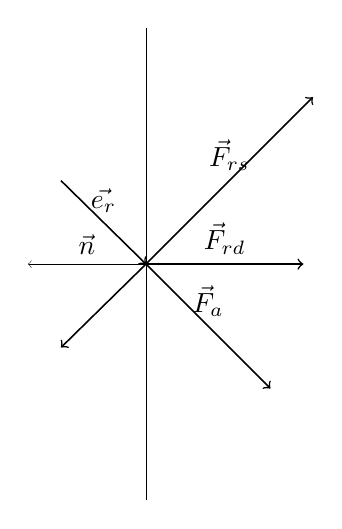
\begin{tikzpicture}
      \coordinate (center) at (3, 0);
      \coordinate (norm) at (1.5, 0);
      \coordinate (eR) at (1.92, 1.06);
      \coordinate (revER) at (1.92, -1.06);
      % \coordinate (tau) at (3, -1.5);

      \coordinate (Fa) at (4.58, -1.58);
      \coordinate (Frs) at (5.12, 2.12);
      % \coordinate (Fe) at (6, 0);
      \coordinate (Frd) at (5, 0);


      \draw[line width=0.05mm, -] (3, -3) -- (3, 3);
      \draw[line width=0.05mm, ->] (center) -- node[above] {$\vec{n}$} (norm);
      \draw[line width=0.2mm, ->] (eR) -- node[above] {$\vec{e_r}$} (center);
      \draw[line width=0.2mm, ->] (center) -- (revER);
      % \draw[line width=0.2mm, ->] (center) -- node[left] {$\vec{\tau}$} (tau);

      \draw[line width=0.2mm, ->] (center) -- node[above] {$\vec{F}_a$} (Fa);
      \draw[line width=0.2mm, ->] (center) -- node[above] {$\vec{F}_{rs}$} (Frs);
      % \draw[line width=0.2mm, ->] (center) -- node[below] {$\vec{F}_e$} (Fe);
      \draw[line width=0.2mm, ->] (center) -- node[above] {$\vec{F}_{rd}$} (Frd);
    \end{tikzpicture}
    \caption{Отражение света солнечным парусом}
    \label{fig:SailLightReflection}
  \end{figure}\par
  Результирующей силой солнечного света будет являться суперпозиция всех указнных выше сил:
  \begin{equation}
    \begin{aligned}
      &\vec{F} = \vec{F}_a + \vec{F}_{rs} + \vec{F}_{rd} \\
      &\vec{F} = -P\Omega\cdot [
      (2|\vec{e}_r\cdot\vec{n}|\rho_s + B_f\rho_d + \gamma\mu)
      (\vec{e}_r\cdot\vec{n})\vec{n} +
      |\vec{e}_r\cdot\vec{n}|(\rho_d + \mu)\vec{e}_r],\\
      & \text{где } \gamma = \frac{\epsilon_fB_f - \epsilon_bB_b}{\epsilon_f + \epsilon_b}
    \end{aligned}
  \end{equation}\par
  Момент силы, возникающий при наличии смещения $d$ центра масс от центра давления
  вдоль нормали паруса, вычисляется как
  \begin{equation}
    T_s = -d\cdot\vec{n}\times\vec{F} = -P\Omega d(\rho_d + \mu) |\vec{e}_r \cdot \vec{n}|\vec{e}_r \times \vec{n}
  \end{equation}
  \subsection{Земная тень}
  ...
\end{document}
